\subsubsection{Create Session}

\begin{figure}[H]
	\begin{subfigure}{0.80\linewidth}
		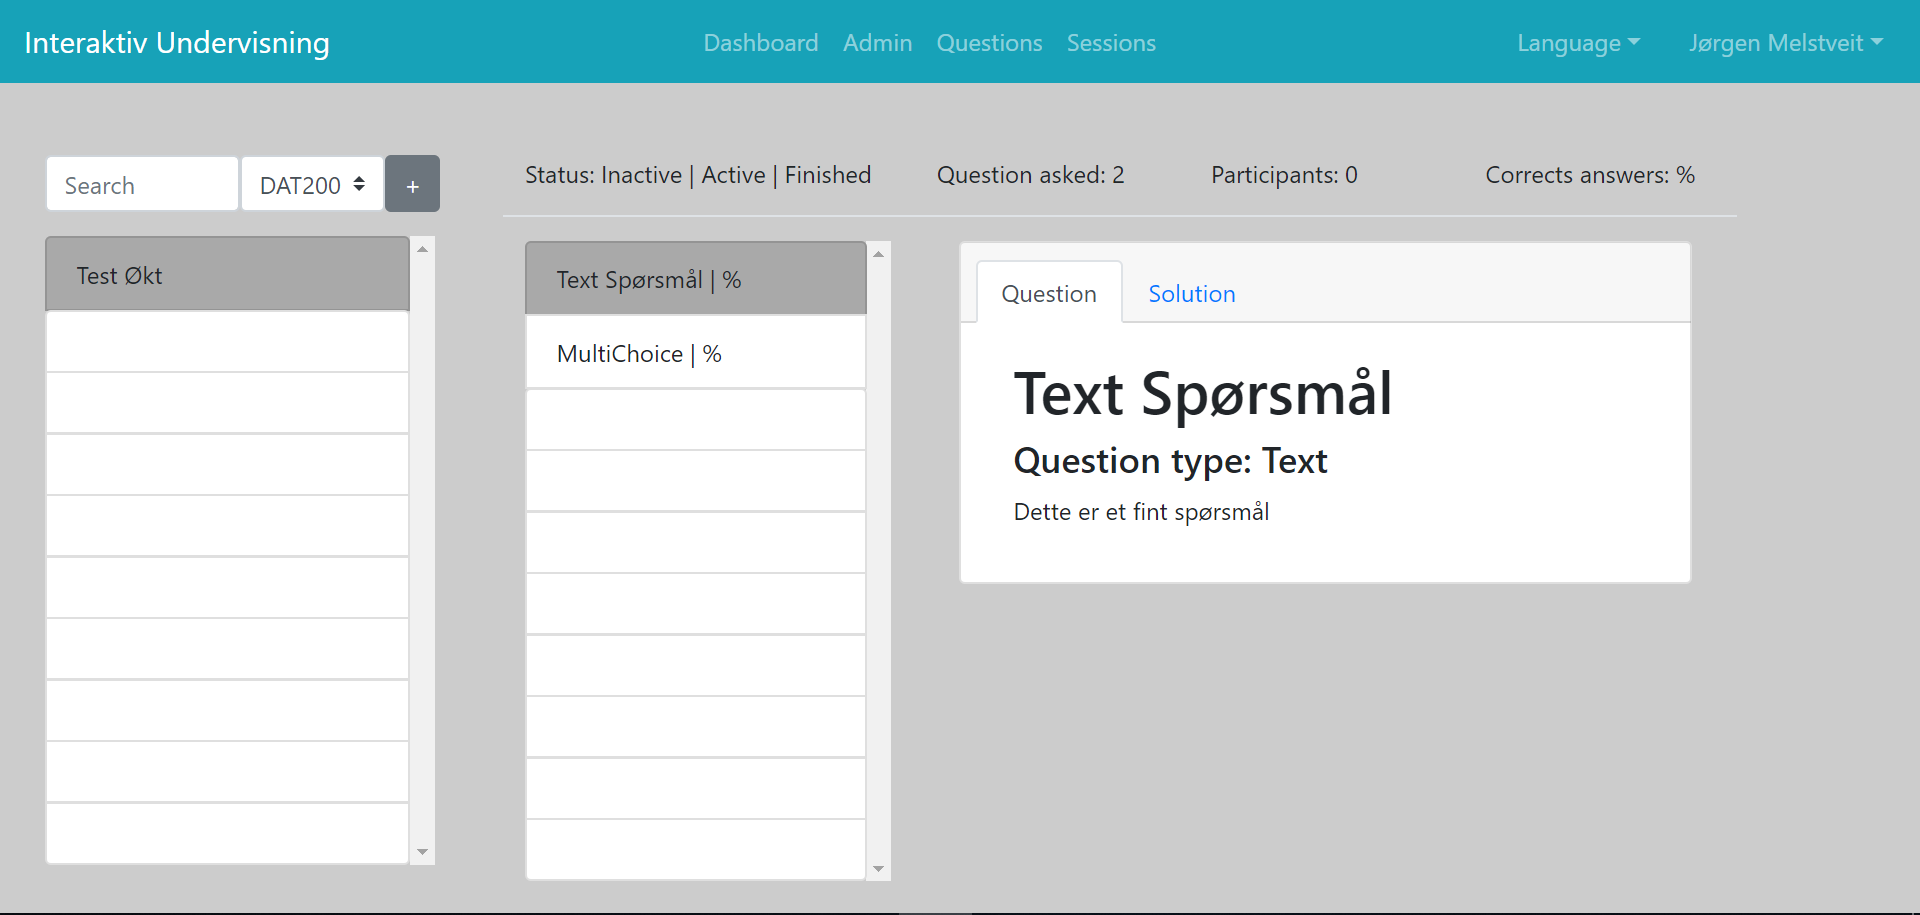
\includegraphics[width=\linewidth]{/userManual/admin/sessionPage}
		\caption{}
		\label{fig:sessionPage}
	\end{subfigure}
	\begin{subfigure}{0.70\linewidth}
		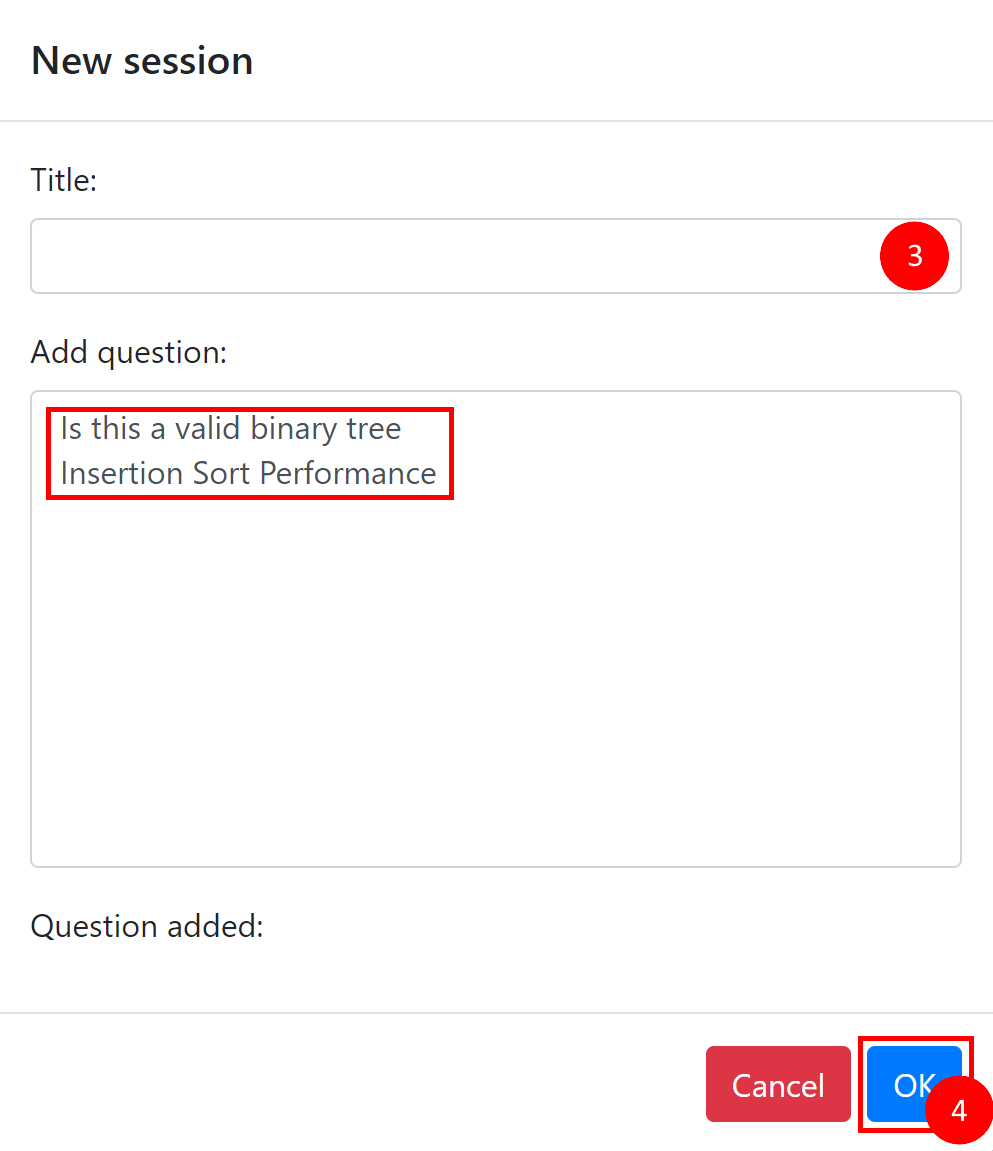
\includegraphics[width=\linewidth]{/userManual/admin/createSession}
		\caption{}
		\label{fig:createSession}
	\end{subfigure}
\end{figure}

\begin{userManualItemlist}
	\item[Step I.] Navigate to the sessions page.
	\item[Step II.] Choose the course you want to create a session for. (1) (Figure: \ref{fig:sessionPage})
	\item[Step II.] Click the "+" button (2) to create new session. (Figure: \ref{fig:sessionPage})
	\item[Step III.] Type in the session's title in the input field marked with "Title" (3). (Figure: \ref{fig:createSession})
	\item[Step IV.] In the "Add question" section, select the questions you want to add the session. (Figure: \ref{fig:createSession})
	\item[Step V.] Verify in "Question added" the questions you want in the session are displayed. (Figure: \ref{fig:createSession})
	\item[Step VI.] Click the "OK" button (4) to create the session. (Figure: \ref{fig:createSession})
	\item[Step VII.] The newly created session should now be in the sessions section on the session page. (Figure: \ref{fig:sessionPage})
\end{userManualItemlist}